Para la problemática presentada anteriormente presentamos en esta sección: el objetivo, objetivos específicos, la justificación, el alcance y la descripción de la propuesta de solución.\\

%Definir correspondencia
%introduccion 
\section{Objetivo}

Para mitigar las causas y reducir el impacto de los problemas que se tienen nos basamos en el siguiente objetivo: \\

Desarrollar e implementar una aplicación web que apoye a las tareas de recepción y entrega de correspondencia interna y externa del CMPL. \\

\subsection{Objetivos Específicos}

\begin{itemize}
	\item Ayudar al personal del CMPL a cumplir los líneamientos establecidos. %cuales 
	\item Que la aplicación apoye a la consulta de correspondencia entrante y saliente.
	\item Que la aplicación envíe notificaciones al destinatario.
	\item Que la aplicación apoye a ver el seguimiento de los asuntos que se deben atender.
\end{itemize}

Para dejar de una manera más clara los objetivos mencionados, en la siguiente sección se presenta una juestificación breve.

\section{Justificación}

Con este trabajo se mitigarán las causas de algunos de los problemas mencionados en el capítulo anterior como: 
%de la siguiente manera || la aplicacion apoyará a: 
\begin{itemize}
	\item Que el registro de la correspondencia se lleve de manera adecuada.
	\item La aplicación resguarde los registros de la correspondencia.
	\item Que se restrinja el acceso a la información al personal indicado.
	\item Que se pueda saber a quien se le turna un oficio y a quien se le envía copia.
	\item Saber el momento en que se respondió.
	\item Saber si requiere respuesta.
	\item Saber si el asunto ya fue atendido. 
	\item Saber quien lo entregó.
	\item Saber quien lo registró.
	\item Informar a la persona que se le turna que tiene un asunto por atender.
	\item Que los oficios sean validados.
	\item Saber la ubicación física de los oficios. 
	\item Cumplir con la normatividad.
\end{itemize}  
Pero sí continua, el rezago tecnológico va a ser necesario que el CMPL adquiera nuevos equipos y que capacite a su personal. \\

De acuerdo con anterior es necesario que para el desarrilo del presente trabajo se defina el alcance que tendrá, el cual se describe en la siguiente sección. 

\section{Alcance}

Para presentar de mejor manera el alcance de la aplicación se divide de la siguiente manera: \\

\begin{itemize}
	\item Funcionalidad: muestra los módulos por los que estará formado la aplicación y los diferentes tipos de usuarios que la utilizarán.
	\item Plataforma: el hardware, el software y los servicios necesarios para la aplicación.
	\item Procedimiento: descripción y mejoras al procedimiento anterior.
	\item Información: la información que se va a manejar dentro de la aplicación.
	\item Propiedades de software: son los atributos con los que contará la aplicación.
	\item Interacción con el usuario: la forma en que el usuario podrá hacer el intercambio de información con la aplicación.
\end{itemize}

%%%%%%%%%% FUNCIONALIDAD %%%%%%%%%%%%
%%%%%%%%%%%%%%%%%%%%%%%%%%%%%%%%%%%%%

\subsection{Funcionalidad}

La funcionalidad la aplicación se organizará de la siguiente manera: un módulo para la gestión de usuarios, un modulo para la correspondencia interna y un módulo para la correspondencia externa. En la figura \ref{diagrama a bloques} se puede ver de manera general como interactuan los bloques anteriores con los diferentes tipos de usuarios.\\

	\begin{figure}[htbp!]
		\centering
			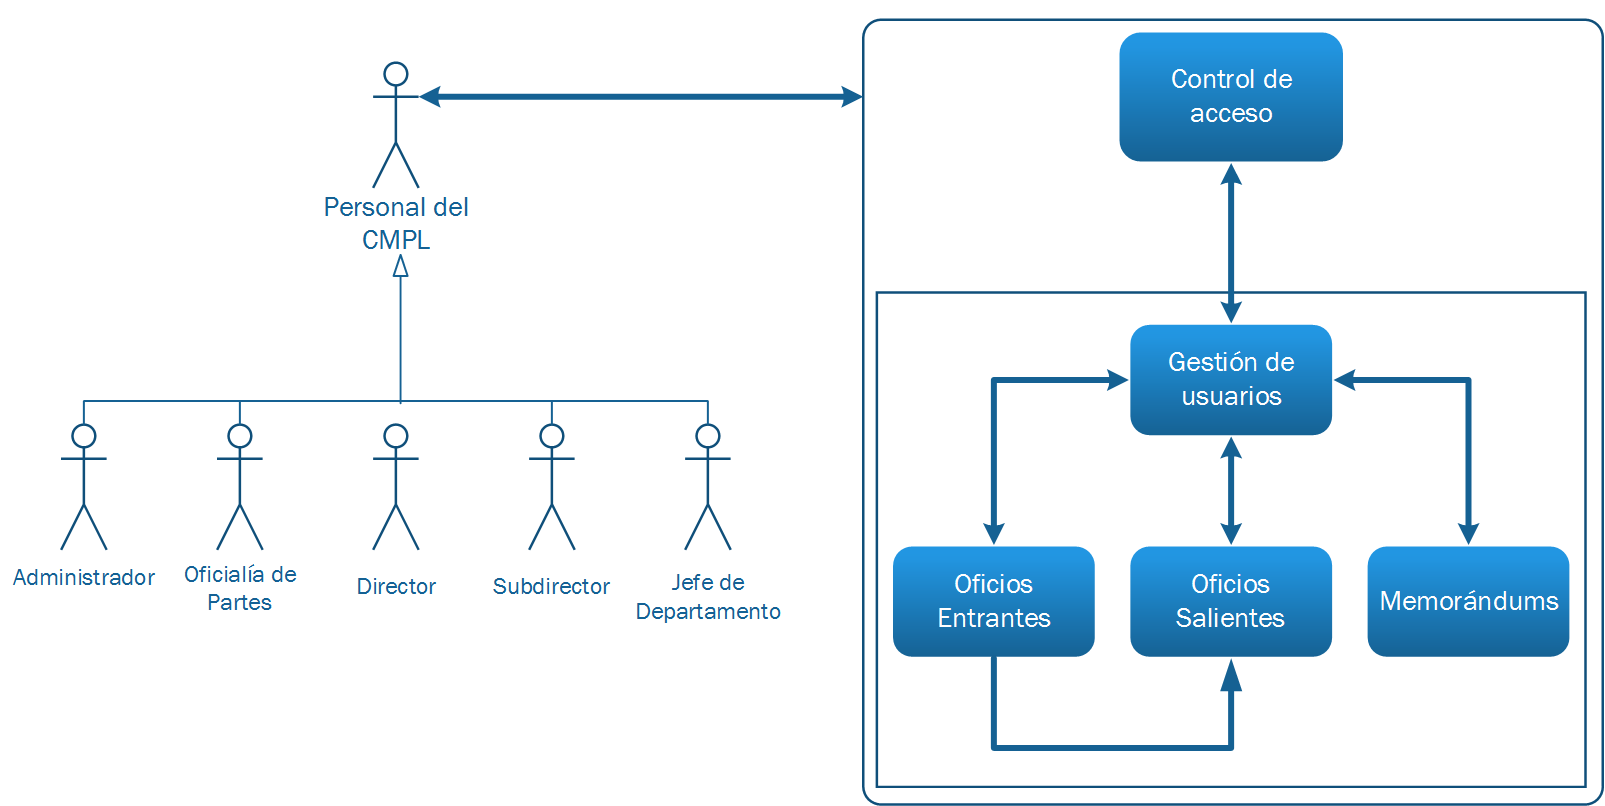
\includegraphics[width=0.8\textwidth]{images/propuesta/diagramabloques}
		\caption{Diagrama de Bloques de la Aplicación.}
		\label{diagrama a bloques}
	\end{figure}

De acuerdo con la figura anterior, a continuación se describe cada módulo:

\subsubsection{Módulo 1: Gestión de usuarios}
Este modulo permitirá el proceso de creación de usuarios, esto es: hacer cambios, dar una contraseña inicial y dar de baja. Es importante tener que cada usuario tenga una cuenta porque una cuenta de usuario hace posible que: se controle el acceso a la información y autentificar la identidad de la persona que ingresa. \\
%todos los usuarios requieren este si no no lo pueden usar

Las consideraciones para este módulo son los siguientes:
\begin{itemize}
	\item El usuario requerirá tener una nombre de usuario y una contraseña porque requiere que se cuide la privacidad de la información. De lo contrario no podrá utilizar la aplicación.
	\item El usuario necesita editar sus datos.
	\item El usuario necesita un mecanismo para recuperar su contraseña.
	\item El usuario necesita registrar nuevos usuarios.
	\item El usuario necesita dar de baja a los usuarios.
	\item El usuario necesita consultar a los usuarios registrados.
	\item La aplicación mostrará las funciones que corresponden de acuerdo al tipo de usuario que ingrese.
\end{itemize} 

Los requerimientos funcionales que implementa este módulo son:
\begin{itemize}
	\item[RF] El usuario podrá autenticarse en la aplicación.
	\item[RF] El usuario podrá cambiar su contraseña.
	\item[RF] El usuario podrá modificar sus datos.
	\item[RF] El usuario podrá registrar nuevos usuarios.
	\item[RF] El usuario podrá dar de baja a usuarios registrados.
	\item[RF] El usuario podrá consultar los usuarios registrados.
\end{itemize}

Con las consideraciones y los requerimientos anteriores se resuelve que el usuario sólo acceda a la información que le corresponda con las funciones que le correspondan.

\subsubsection{Modulo 2: Correspondencia Externa}
Este modulo permitirá el registro, la consulta de la correspondencia que llega al CMPL. \\

Las consideraciones para este módulo son los siquientes:

\begin{itemize}
	\item El usuario necesita una herramienta para registrar la correspondencia de manera más controlada.
	\item El usuario necesita subir el oficio en formato digital.
	\item El usuario necesita consultar los oficios respondidos.
	\item El usuario necesita consultar el momento en que un oficio fue entregado.
	\item El usuario necesita turnar el oficio.
	\item El usuario necesita enviar una copia del oficio.
	\item El usuario necesita saber a quien se le turno un oficio.
	\item El usuario necesita saber si un oficio requiere respuesta.
	\item El usuario necesita descargar un oficio.
	\item El usuario necesita dar respuesta a un oficio.
	\item El usuario necesita asignar carácter al oficio.
	\item La aplicación mostrará el registro del oficio.
	\item La aplicación mostrará los oficios pendientes.
	\item La aplicación mostrará los oficios respondidos.
	\item La aplicación mostrará el estátus del oficio.
\end{itemize}

Los requerimientos funcionales que implementa este modulo son: 

\begin{itemize}
	\item[RF] El usuario podrá registrar oficios entrantes.
	\item[RF] El usuario podrá guardar el documento escaneado.
	\item[RF] El usuario podrá enviar una copia.
	\item[RF] El usuario podrá cancelar el proceso de la correspondencia.
	\item[RF] El usuario podrá registrar anexos.
\end{itemize}

Con esto se resuelve la problemática para la los oficios entrantes se lleve de manera adecuada el resgistro, se tenga un respaldo y se le pueda dar el seguimiento. 

\subsubsection{Modulo 3: Correspondencia Interna}
Este modulo permitirá el registro, la consulta y el seguimiento de los memorándums dentro del CMPL.\\

Los requerimientos considerados para este módulo son los siguientes: 
\begin{itemize}
	\item El usuario necesita registrar memorándums.
	\item El usuario necesita subir el memorándum.
	\item El usuario necesita turnar el memorándum.
	\item El usuario necesita envíar copia del memorándum.
	\item El usuario necesita asignar prioridad al memorándum.
	\item El usuario necesita consultar los memorándums. 
\end{itemize}

Los requerimientos funcionales que implementa este modulo son: 

\begin{itemize}
	\item[RF] El usuario podrá registrar memorándums.
	\item[RF] El usuario podrá guardar el documento escaneado.
	\item[RF] El usuario podrá enviar una copia.
	\item[RF] El usuario podrá cancelar el proceso de la correspondencia.
	\item[RF] El usuario podrá registrar anexos.
\end{itemize}

%De acuerdo con los requerimientos anteriores se resuelve que: los oficios tengan un respaldo, que se sepa el estatus de un oficio, que se lleve de manera correcta el registro de los oficios y que se le notifique al usuario que ha recibido correspondencia.\\
%En cuanto a los tipos de usuarios que utilizarán la aplicación, cada uno tiene responsabilidades diferentes en el CMPL por lo tanto dentro de la aplicación sus funciones serán diferentes y se describen a continuacion: \\

%%%%%%%%%%%%%%%%%%%%%%%%%%%%%%%%%%%%%%%%%%%%%
%%%%%%%%%%%%%%%%%ROLES DE USUARIOS%%%%%%%%%%%

\subsection{Descripción de roles de usuarios}
En esta sección se presentan y describen cada uno de los posibles perfiles de usuarios que tenemos para la aplicación, en ellos se estará dividiendo el control de acceso a la misma como se lista a continuación.\\

\subsubsection{Administrador}
Es el jefe del Departamento de Sistemas y Banco de Datos del CMPL. Tiene el control total de la administración de la información mostrada en la aplicación web.\\

\textbf{Responsabilidades:}
\begin{itemize}
	\item Dar de alta nuevos usuarios.
	\item Editar usuarios existentes.
	\item Eliminar usuarios.
	\item Registrar correspondencia saliente (oficios y memorándums).
	\item Consultar correspondencia.
	\item Dar seguimiento a su correspondencia.
\end{itemize}

\subsubsection{Oficialía de Partes}
Es la persona que lleva a cabo la recepción de correspondencia formal del CMPL. Recibe los documentos de correspondencia y los registra en una bitácora; firma y sella de recibido y turna los oficios y memos a sus respectivos destinatarios.\\

\textbf{Responsabilidades:}
\begin{itemize}
	\item Verificar que los documentos recibidos cumplan con todos los lineamientos requeridos para su recepción.
	\item Registrar la correspondencia formal interna y externa del CMPL.
	\item Turnar los oficios y memorándums a sus respectivos destinatarios.
	\item Registrar correspondencia saliente.
\end{itemize}

\subsubsection{Personal CMPL}
Es un trabajador del CMPL registrado en el directorio, que no es Jefe del Departamento de Sistemas y Banco de Datos o encargado de Oficialía de Partes.\\

\textbf{Responsabilidades:}
\begin{itemize}
	\item Checar su correspondencia entrante.
	\item Registrar correspondencia saliente.
	\item Turnar correspondencia.
	\item Recibir correspondencia.
	\item Atender observaciones\footnote{Se entiende por observaciones aquellas indicaciones que deben ser atendidas} a los oficios registrados.
\end{itemize}

\subsubsection{Director}
Es un trabajador del CMPL con el nombramiento de “Director”. Es la persona que representa al centro ante otras dependencias. Se encarga de administrar y gestionar las decisiones importantes del centro junto con su grupo de trabajadores.\\

\textbf{Responsabilidades:}
\begin{itemize}
	\item Turnar oficios entrantes.
	\item Turnar copia de oficios entrantes.
	\item Firmar oficios salientes.
	\item Cancelar proceso de oficios entrantes.
	\item Cancelar proceso de oficios salientes.
	\item Ver detalles de correspondencia.
	\item Responder oficios.
\end{itemize}

\subsubsection{Jefe de Departamento}
Es un trabajador del CMPL que está como encargado de alguna de las diferentes jefaturas que existen en el centro. Se encarga de apoyar a la dirección con las decisiones importantes para el CMPL y de atender los asuntos que conciernen con el departamento del cual está encargado.\\

\textbf{Responsabilidades:}
\begin{itemize}
	\item Atender correspondencia a nombre del director.
	%\item Manejar los indicadores mensuales.
	\item Cancelar proceso de correspondencia saliente.
	\item Generar oficios salientes nuevos.
	\item Dar respuesta a oficios entrantes.
	\item Atender observaciones a los oficios registrados.
\end{itemize}

\subsubsection{Subdirector}
Es un trabajador del CMPL que esta como encargado en alguna de las subdirecciones existentes dentro del centro. Se encarga de las decisiones que conciernen al área y de la administración de dicho departamento. Puede que tenga a su cargo otra jefatura y debe trabajar en conjunto con esta otra área.\\ 

\textbf{Responsabilidades:}
\begin{itemize}
	\item Responder oficios entrantes.
	\item Registrar oficios salientes.
	\item Turnar correspondencia en caso de que tenga alguna jefatura a su cargo.
	\item Ver detalles de correspondencia.
	\item Atender observaciones a los oficios registrados.
\end{itemize}

De acuerdo con los usuarios y módulos anteriores se requiere que el CMPL cuente con una plataforma para que la aplicación pueda operar dicha plataforma se muestra a continuación.
%y para que esto sea posible se realizó un estudio de factibilidad de los recursos técnicos necesarios para su funcionamento. \\

%%%%%%%%%% PLATAFORMA %%%%%%%%%%%%%%%
%%%%%%%%%%%%%%%%%%%%%%%%%%%%%%%%%%%%%
%\subsection{Estudio de Factibilidad}

\subsection{Plataforma}

Para que la aplicación funcione se necesita de los componentes de hardware, software y los servicios. En la figura \ref{arquitectura} se puede ver de una manera general como interactuan estos componentes. \\

\begin{figure}[htbp!]
		\centering
			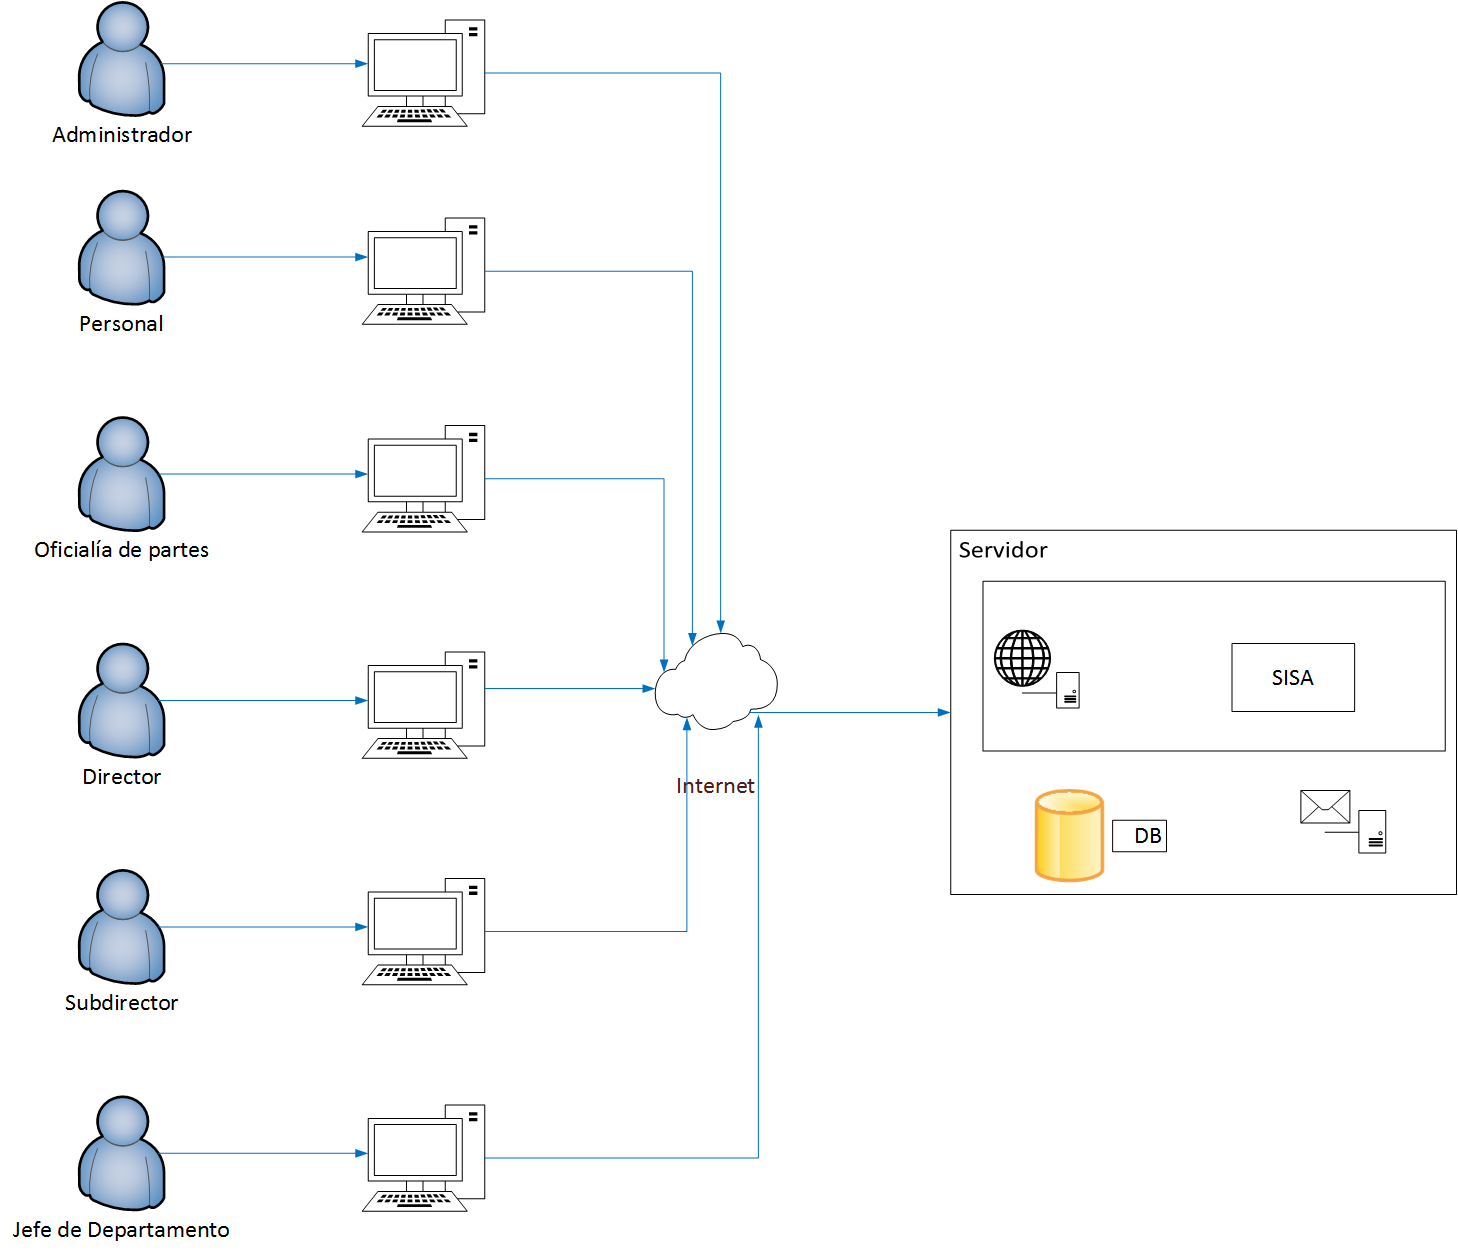
\includegraphics[width=0.8\textwidth]{images/propuesta/arquitectura}
		\caption{Arquitectura de la Aplicación.}
		\label{arquitectura}
	\end{figure}

\subsubsection{Hardware}

Dentro del hardware el CMPL actualemnte cuenta con:
\begin{enumerate}
	\item Un servidor que de el servicio a las computadoras, aloje la aplicación así como los registros de la correspondencia y se hagan los respaldos. Este servidor deberá contar con: 
	\begin{itemize}
		\item Al menos con 500 GB de disco duro.
		\item Un monitor.
		\item Un teclado.
		\item Un mouse.
		\item Al menos 8 GB en memoria RAM.
		\item Un procesador Intel Xeon.
	\end{itemize}
	\item Cada trabajador deberá contar con una computadora ya sea de escritorio o laptop con: 
	\begin{itemize}
		\item Al menos 256 GB de disco duro.
		\item 2 GB en memoria RAM.
		\item Un procesador Intel Quad Core. 
	\end{itemize}
\end{enumerate}

\subsubsection{Software}
El software que requiere es: 
\begin{enumerate}
	\item Un sistema operativo tanto para el servidor como las computadoras.
	\item Un navegador de internet.
	\item Un gestor de base de datos.
	\item Un servidor de correos.
	\item Un servidor web.
\end{enumerate}
\subsubsection{Servicios}

Por último se requiere de los siquientes servicios: 
\begin{itemize}
	\item Energía eléctrica para el funcionamiento
	\item Una planta de luz para que cuando se vaya la luz el servidor siga operando.
	\item Un sistema de enfriamiento para refrigeración del servidor y evitar averias.
	\item Site para colocar el servidor.
	\item Una puerta con llave para que ninguna persona diferente al jefe del departamento de sistemas y banco de datos entre y modifique la configuración del servidor.
	\item Que el administrador genere respaldos.
	\item Cámaras de seguridad. 
	\item Servicio web para que los usuarios accedan a la aplicación. 
	\item Configuración de red.
\end{itemize} 

%De acuerdo con los componentes mencionados anteriormente se ...
%%%%%%%%%% PROCEDIMIENTO %%%%%%%%%%%%
%%%%%%%%%%%%%%%%%%%%%%%%%%%%%%%%%%%%%
\subsection{Procedimiento}
Con esta propuesta se mejora el procedimiento presentado en el capitulo 1, las principales mejoras son:

\begin{itemize}
	\item Alertas al usuario: cuando el usuario este utilizando la aplicación está mostrará los asuntos que no ha atendido. 
	\item Notificaciones al correo: una vez que se turne un oficio, se enviará un correo electrónico al usuario diciendo que tiene un nuevo asunto por atender. 
	\item Respaldos: el administrador podrá realizar los respaldos de todos los registros de la corespondencia así como los documentos digitales.
	\item Seguimiento: el seguimiento de la correspondencia se refiere a si ya fue atendido, si está en atención, si fue respondido o si está enterado.
\end{itemize}

\subsubsection{Oficios entrantes}

En la figura \ref{Registro oficio} se muestra cómo sería el proceso de registro de oficios con la aplicación.

\begin{figure}[htbp!]
		\centering
			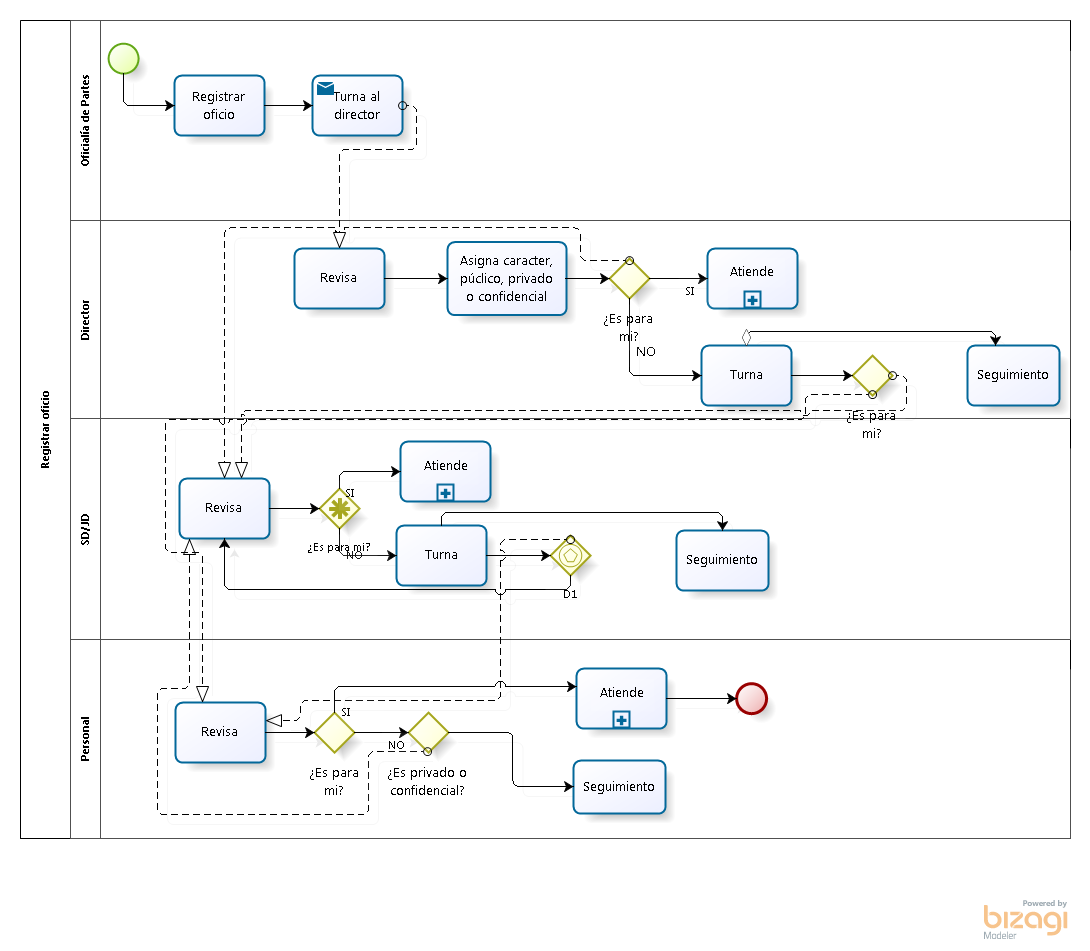
\includegraphics[width=0.8\textwidth]{images/propuesta/registrooficio}
		\caption{Procedimiento de recepción.}
		\label{Registro oficio}
	\end{figure}

\begin{enumerate}
	\item Oficialía de partes registrará el oficio en la aplicación.
	\item Oficialía de partes escanea el documento y guarda el registro. 
	\item Oficialía de partes turnará al director.
	\item La aplicación notificará al director.
	\item El director lo revisa el oficio y ve si es para el.
	\item Si es para él lo atiende.
	\item Si no asigna el caracter del oficio (público, privado o confidencial).
	\item Si es confidencial turna directamente al destinatario. 
	\item El destinatario recibe y verifica que sea para él.
	\item Si es para él, atiende el oficio.
	\item Si no, entonces regresa al Director.
	\item Si el oficio no es confidencial entonces el Director turna al Subdirector o Jefe correspondiente.
	\item Éste lo revisará y si es para él lo atiende, si no lo turna al personal.
	\item El personal lo revisa y verificará si es para él para atenderlo.
	\item Si no tendrá que ver el si es privado o confidencial y regresarlo a su jefe inmediato.
\end{enumerate}

\subsubsection{Respuesta oficios}

En la figura \ref{Procedimiento respuesta} se muestra cómo sería el proceso de registro de oficios con la aplicación.

\begin{figure}
	\centering 
		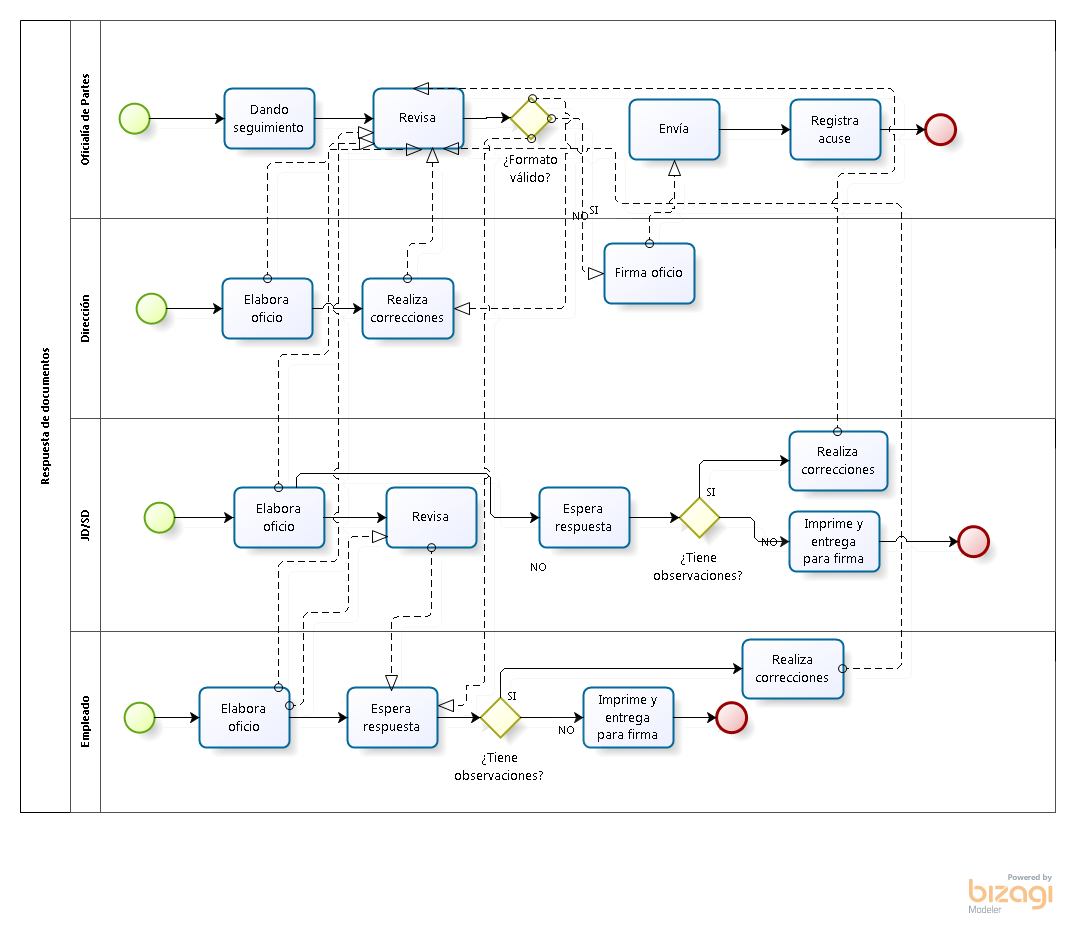
\includegraphics[width=0.8\textwidth]{images/propuesta/procesorespuesta}
	\caption{Procedimiento respuesta.}
\end{figure}

Con esto se tiene la información general que se podrá manejar dentro de la aplicación, la cual se describe en la siguiente sección.

%%%%%%%%%% INFORMACION %%%%%%%%%%%%%%
%%%%%%%%%%%%%%%%%%%%%%%%%%%%%%%%%%%%%
\subsection{Información}

Para la información a manejar dentro de la aplicación de manera general se comtempla manejar la información de:
\begin{itemize}
	\item Usuarios: Nombre completo, departamento al que pertenece, rol que desempeña dentro de la aplicación, contraseña y correo electrónico.
	\item Oficio entrante: número de oficio, fecha de redacción, área que emite, emisor, cargo del emisor, destinatario, cargo del destinatario, dependencia, asunto, fecha de acuse, nombre de quien entrega, si requiere o no respuesta, a quien se le turnó, a quien se le envió copia y si tiene documentos adjuntos. Además contará con un selector de archivos que permite la carga del documento escaneado en formato PDF y adjuntarlo al registro.
	\item Oficio saliente: número de oficio, fecha de redacción, área que emite, emisor, cargo del emisor, destinatario, cargo del destinatario, dependencia, asunto, fecha de acuse, nombre de quien entrega, si es respuesta a un oficio anterior y si tiene documentos adjuntos.
	\item Memorándum: fecha de redacción, destinatario, cargo del destinatario, departamento, asunto, área que emite, emisor, cargo del emisor, si require respuesta.  
	\item Dependencias: Nombre de la dependencia y acrónimo de la dependencia.
\end{itemize}

Para los documentos (oficios entrantes, salientes y memorándums) se manejarán a parte, sólo se escanean y se guardan dentro de la aplicación. 

Con toda la información a manejar surgen algunas propiedades a considerar para la operación de la acplicación, dichas propiedades se definen a continuacion.\\

%%%%%%%%%% PROPIEDADES DE SW %%%%%%%%
%%%%%%%%%%%%%%%%%%%%%%%%%%%%%%%%%%%%%
\subsection{Propiedades de software}

Las propiedades de software o propiedad no funcional de un sistema, es una limitación en la manera en que el sistema implementa y emite su funcionalidad; es decir, son restricciones en las funciones que ofrece un sistema. Incluyen restricciones sobre el tiempo, confiabilidad, disponibilidad, seguridad, eficiencia, escalabilidad, tolerancia a fallos y robustes. \\

Para fines de este proyecto sólo se considerará la confiabilidad, la disponibilidad, la robustes y la seguridad debido a que realizar un sistema con todas las propiedades no funcionales resulta muy complejo y requeriría más tiempo del que se dispone para lograse, además de que se acordó con el CMPL que no requiere que lleve todas las propiedades porque el sistema es sólo para operarse dentro del centro. A continuación se define cada una de ellas. \\ %poner un porque acertivo 

\textbf{Seguridad\\}
Indica la capacidad de un sistema de software para evitar fallos que se traducirá en la pérdida de vidas, lesiones, daños significativos a la propiedad o destrucción de la propiedad\cite{Seguridad}.

\textbf{Confiabilidad\\}
La confiabilidad de un sistema es la probabilidad de que el sistema realizará su funcionalidad bajo los limites de diseño especificados, sin fallo, durante un periodo de tiempo determinado\cite{Seguridad}.\\

\textbf{Disponibilidad\\}
La disponibilidad es la probabilidad de que el sistema esta operando en un tiempo particular\cite{Seguridad}.\\ 

\textbf{Robustes\\}
Un sistema de software es robusto si es capaz de responder adecuadamente a las condiciones de tiempo de ejecución no anticipados\cite{Seguridad}.\\

Con respecto a los atributos mencionados anteriormente, la confiabilidad y seguridad nos permitirán garantizar un buen desempeño de la aplicación. La aplicación deberá ser capaz de dar respuesta al acceso de todos los usuarios con un tiempo de respuesta aceptable, en la medida de que el CMPL cuente con la plataforma mencionada, en periodos de alta, media y baja demanda de su uso.\\

En cuanto a la disponibilidad consideramos que la aplicación deberá estar al 100 o lo más cercano durante el horario hábil laboral del CMPL. Así mismo, operar de la misma manera para todos los niveles del organigrama del CMPL.\\
% se considera que el servidor se deberá encontrar en buenas condiciones... 

%%%% INTERACCION CON EL USUARIO %%%%%
%%%%%%%%%%%%%%%%%%%%%%%%%%%%%%%%%%%%%
\subsection{Interacción con el usuario}

La interacción de la aplicación con el usuario será mediante pantallas con formularios, mensajes de confirmación, alertas. Para esto se utlizarán herramientas como JQuery o Ajax porque nos permite simplificar la manera de interactuar con los documentos HTML, manipular las hojas de estilo para dar efectos.
%Cuenta con una pantalla que tiene un formulario de autenticación donde se le solicita al usuario su correo institucional y su contraseña. Cuando el usuario ingresa sus credenciales la aplicación verifica su correo y su contraseña; si existen entonces la aplicación muestra la pantalla principal de acuerdo al tipo de usuario que sea. En caso contrario, la aplicación regresa a la pantalla de autenticación con un mensaje de error diciendo que los datos introducidos no son válidos.

\section{Metodología}

La metodología que se utiliza para el desarrollo de este trabajo es Espiral, la cual consiste en hacer un conjunto de actividades en cada iteración las cuales no tienen prioridad sino que se eligen comenzando por la iteración anterior.\\

Para este proyecto se realizarán 4 iteraciones, en esta primera fase de evaluación se realizaron las primeras dos iteraciones. La primera iteración consistió en investigar y probar  diferentes tecnologías para desarrollar el proyecto tanto hardware como software y una vez hecho se configuraron las máquinas a utilizar y el servidor del CMPL. \\
La segunda iteración se realizó el análisis, diseño y desarrollo de la problemática, se realizaron las primeras pantallas.\\

Por último en la tercera y cuarta iteración se realizará el desarrollo de pantallas funcionales, así como la implementación de la aplicación en el servidor del CMPL, además del manual técnico y la capacitación del personal. \\ 

%\item Que la aplicación controle el acceso de los usuarios restringiendo el uso de aplicación a la información y funciones que le corresponden.